\scanpage{217}
Lien avec la variété des modules pour des motifs polarisés rigidifiés:
si \deleted{\unsure{le}} $\mathcal M$ est une telle variété modulaire, alors un morphisme
\diagram{\begin{tikzcd}[column sep=12pt]X\arrow[r,no head]&\mathcal M\end{tikzcd}}
est déterminé quand on connaît sa valeur \uline{en un point}, plus l'application
\diagram{\begin{tikzcd}[column sep=12pt]\pi_1(X)\arrow[r,no head]&\pi_1(\mathcal M)\end{tikzcd}}
......

C'est une propriété intrinsèque importante de ces $\mathcal M$, et une propriété de cette nature mérite d'être étudiée pour ses propres mérites .....
Peut-être peuvent elles \unsure{toutes} être
\deleted{\unsure{caractérisées}}\inserted{\unsure{interprétées}}
comme des \deleted{\unsure{schémas}}\inserted{variétés} modulaires pour certains types de motifs..

\figure{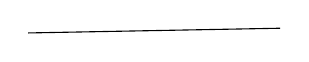
\begin{tikzpicture}\draw (0,0)--(3.2,.06);\end{tikzpicture}}

Introduire la notion de schéma \inserted{motiviquement} ponctué,
\inserted{\figure{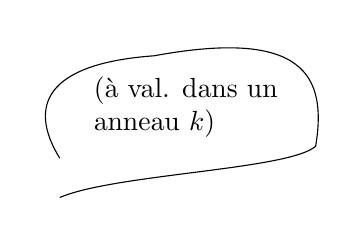
\begin{tikzpicture}[baseline=(a.base)]
\node[align=left] (a) {(\unsure{à val.} dans un\\anneau $k$)};
\draw (-1.6,-.65) .. controls (-2,0) and (-1.8,.55) .. (-.4,.65)
.. controls (1.5,1) and (1.8,.4) .. (1.65,-.5)
.. controls (1.3,-.8) and (-.9,-.85) .. (-1.6,-1.15);
\end{tikzpicture}}}
et morphismes de tels, qui définissent des morphismes correspondants pour les
\diagram{\begin{tikzcd}[column sep=16pt]G(X,\xi)\arrow[r,no head]&G(Y,\eta)\end{tikzcd}},
donc pour
\diagram{\begin{tikzcd}[column sep=18pt]
G(X,\xi)(k)=\pi_1(X,\xi)\arrow[r,no head]&G(Y,\eta)(k)=\pi_1(Y,\eta).
\end{tikzcd}}

\margin{216}
